Para atingir o objetivo deste artigo, foram desenvolvidas duas versões de um mesmo aplicativo de notas, uma utilizando o padrão MVC, e outra utilizando a Arquitetura Limpa.
A aplicação permite o cadastro e autenticação por meio de credenciais ou de uma conta Google.
Após autenticar-se, o usuário é capaz de criar, visualizar, editar e apagar notas que existam em sua conta.
Os dados são armazenados no serviço remoto Firebase \cite{firebase}, além de serem persistidos localmente no dispositivo.
O aplicativo foi construído utilizando a linguagem Dart, fazendo uso do framework Flutter~\cite{flutter}.
Na Figura~\ref{fig:screenshots} é possível visualizar cinco capturas de tela do aplicativo.
A Figura~\ref{fig:project_clean_arch} contém o diagrama da aplicação desenvolvida com a arquitetura limpa, e a Figura~\ref{fig:project_mvc} contém o diagrama da aplicação desenvolvida com MVC.

\begin{figure}[ht]
	\centering
	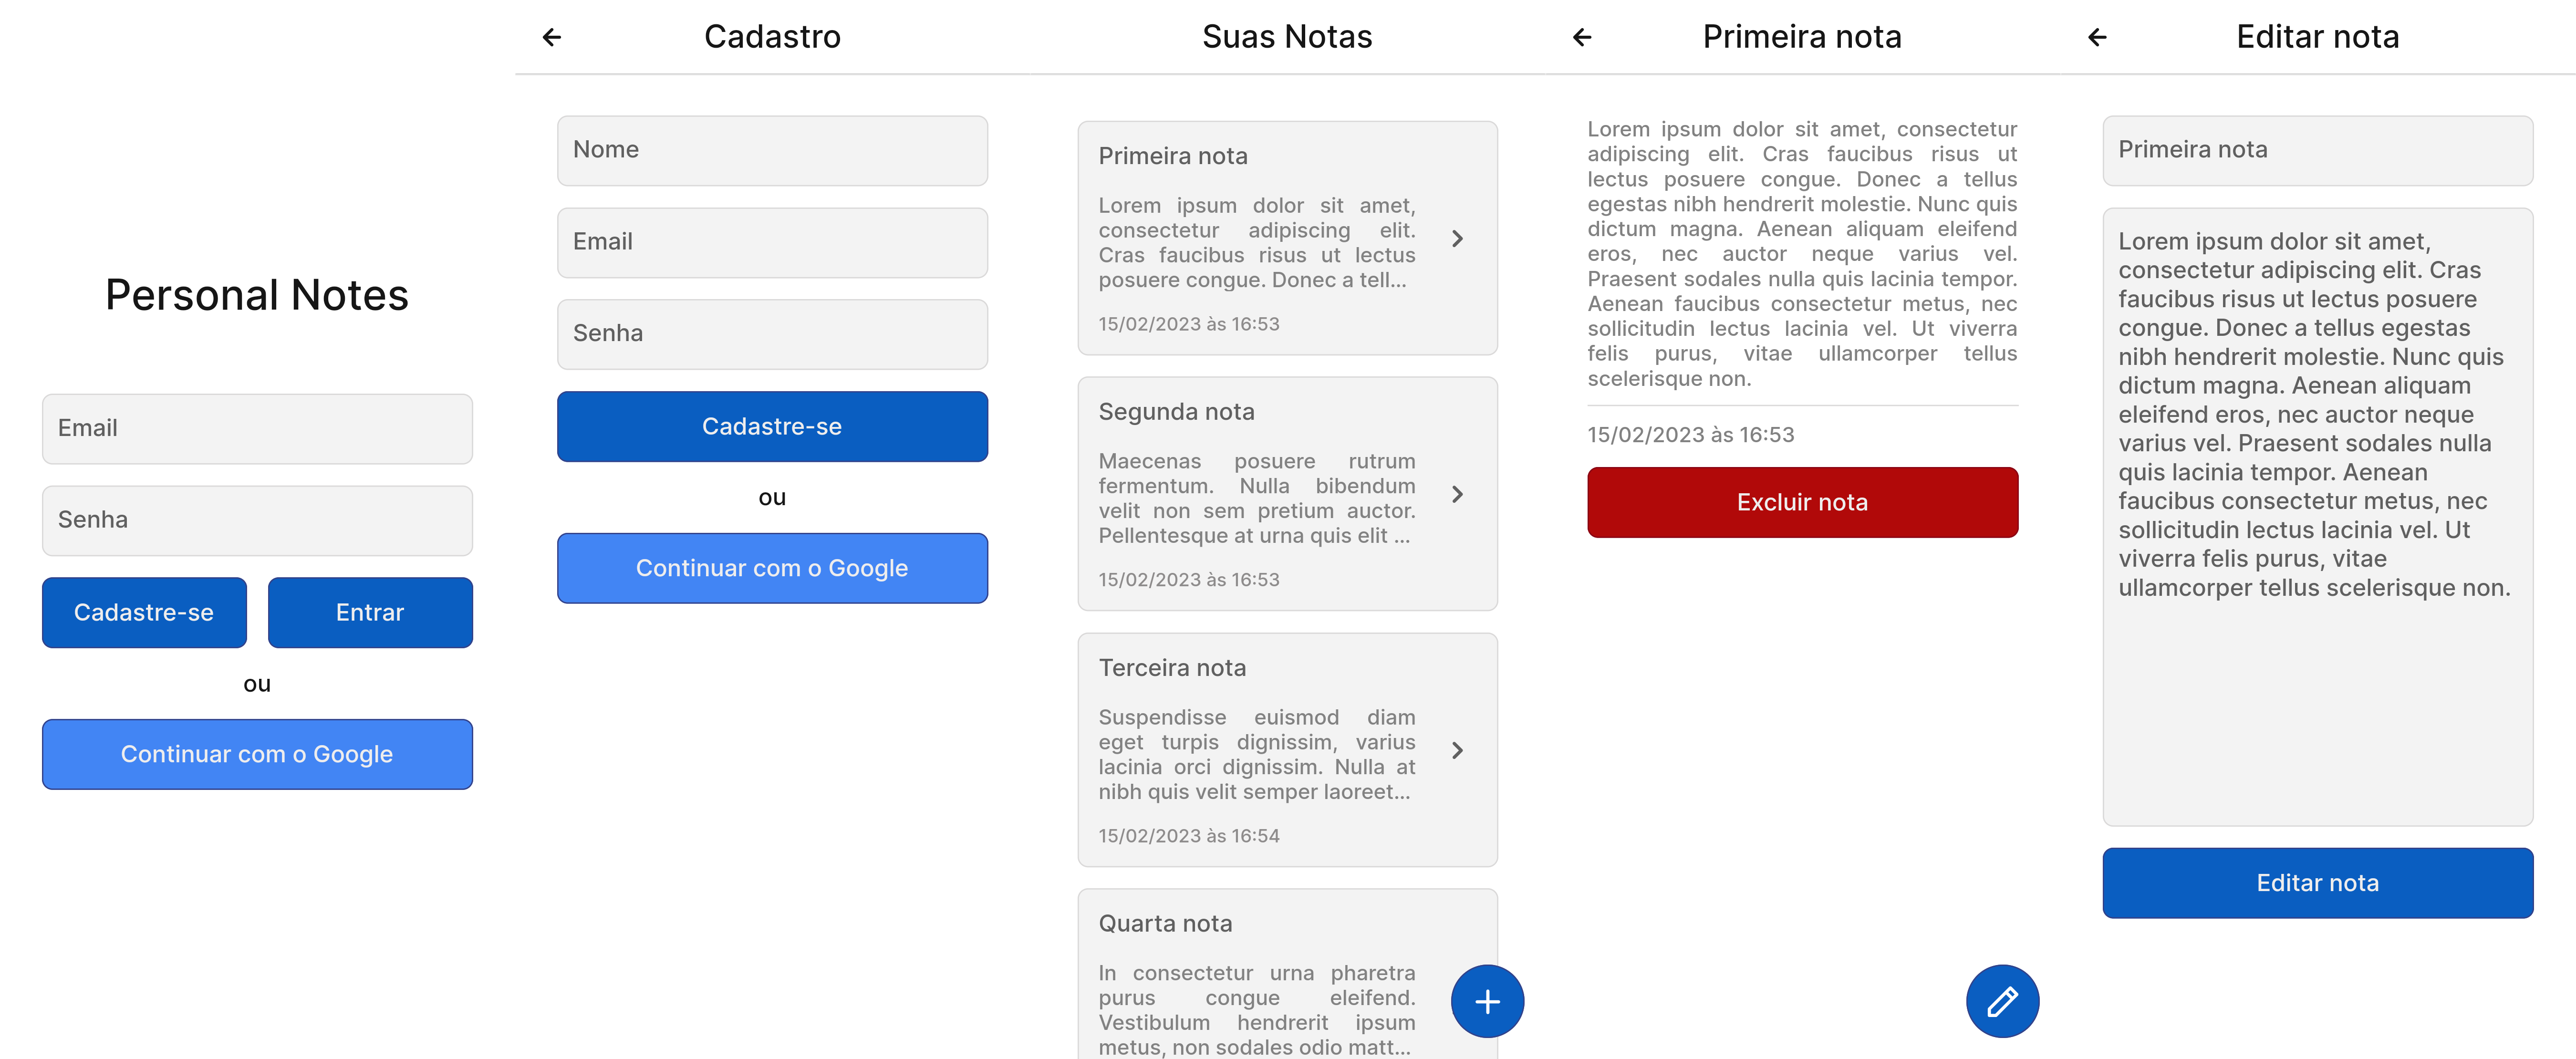
\includegraphics[width=0.9\textwidth]{images/screenshots.png}
	\caption{Capturas de tela do aplicativo}
	\label{fig:screenshots}
\end{figure}

\begin{figure}[ht]
	\centering
	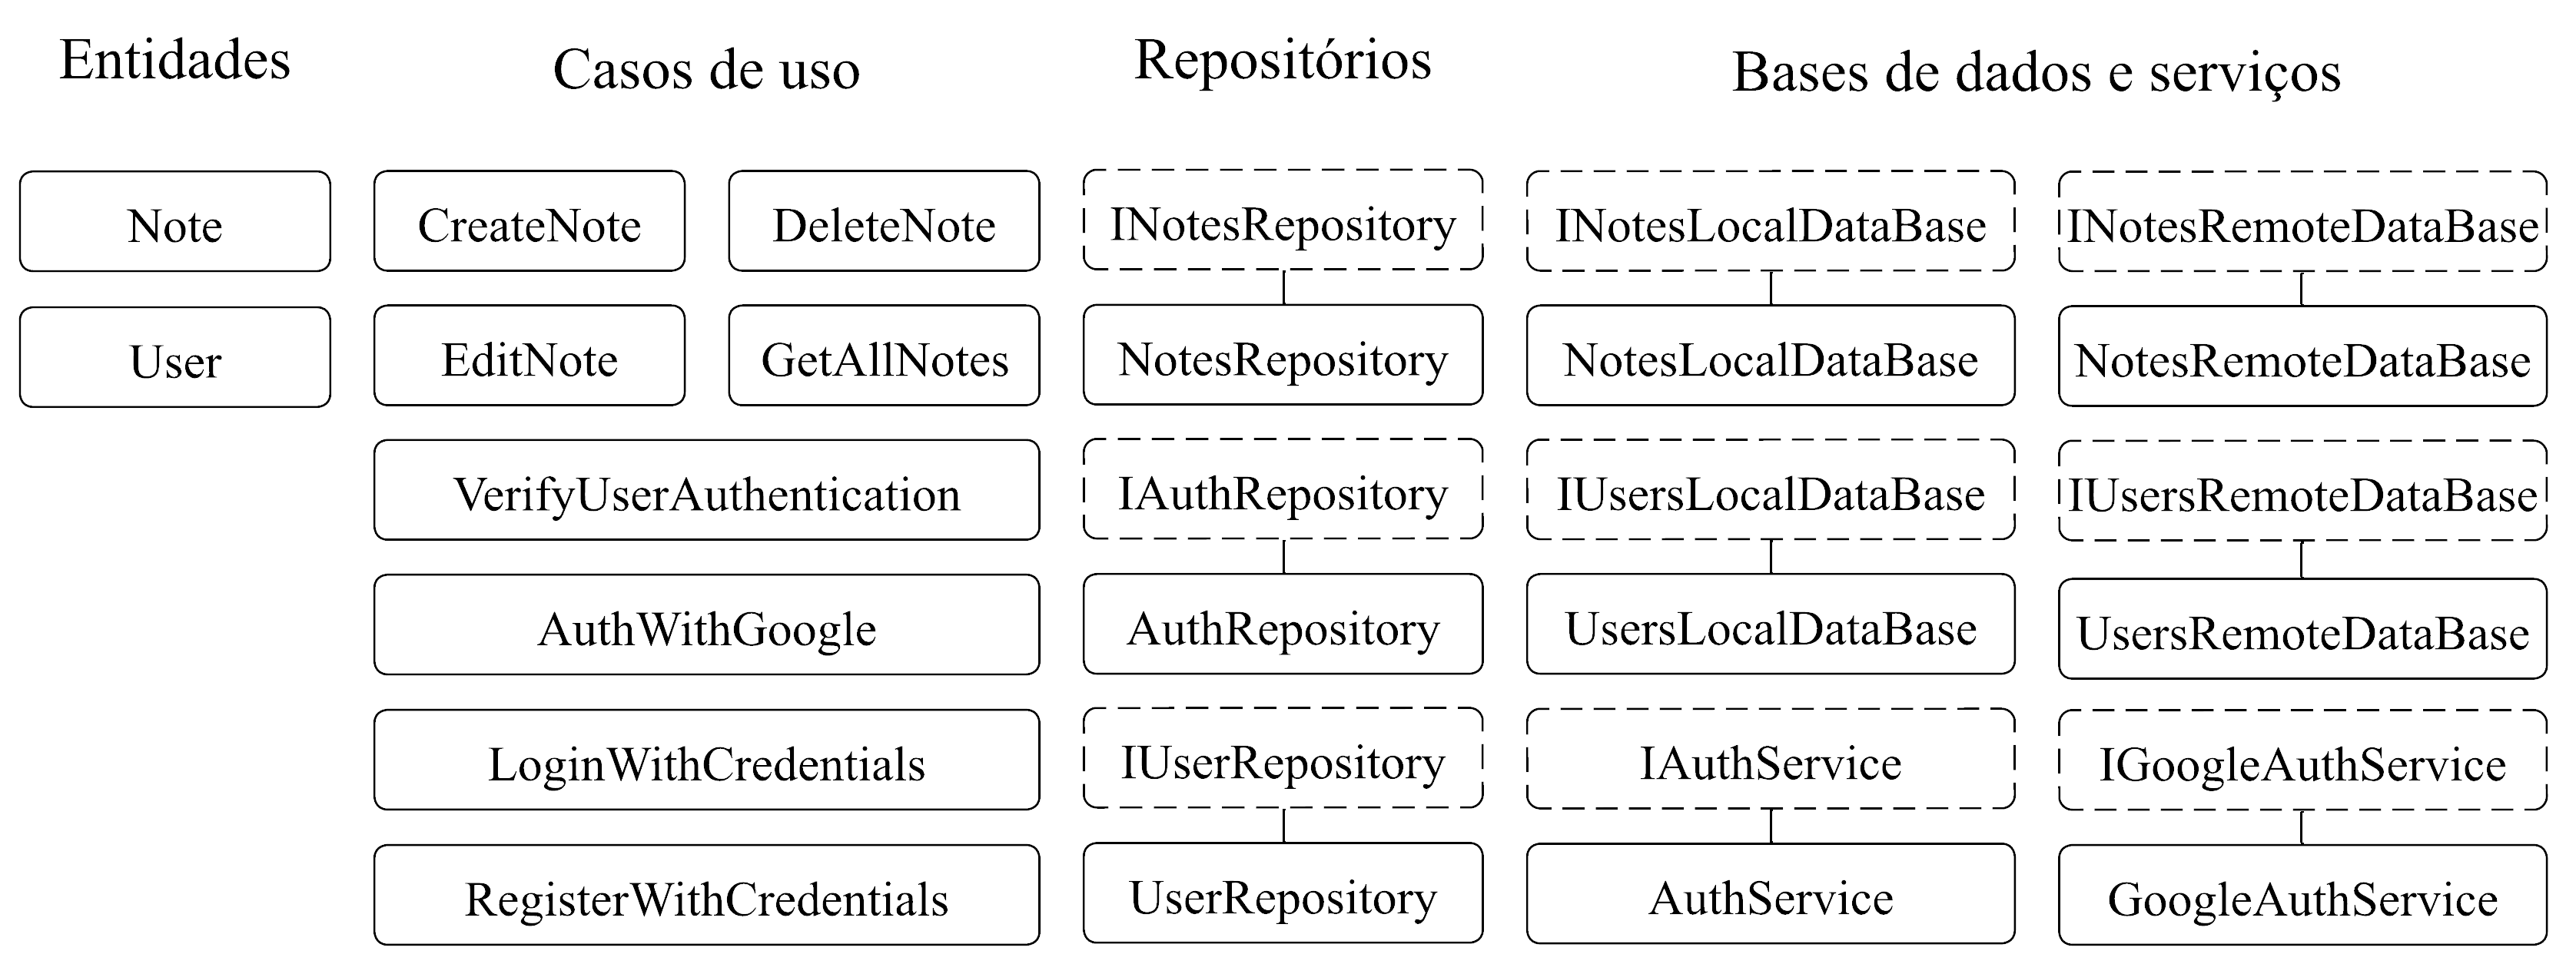
\includegraphics[width=1\textwidth]{images/project_clean_arch.png}
	\caption{Diagrama do projeto criado com a arquitetura limpa}
	\label{fig:project_clean_arch}
\end{figure}

\begin{figure}[ht]
	\centering
	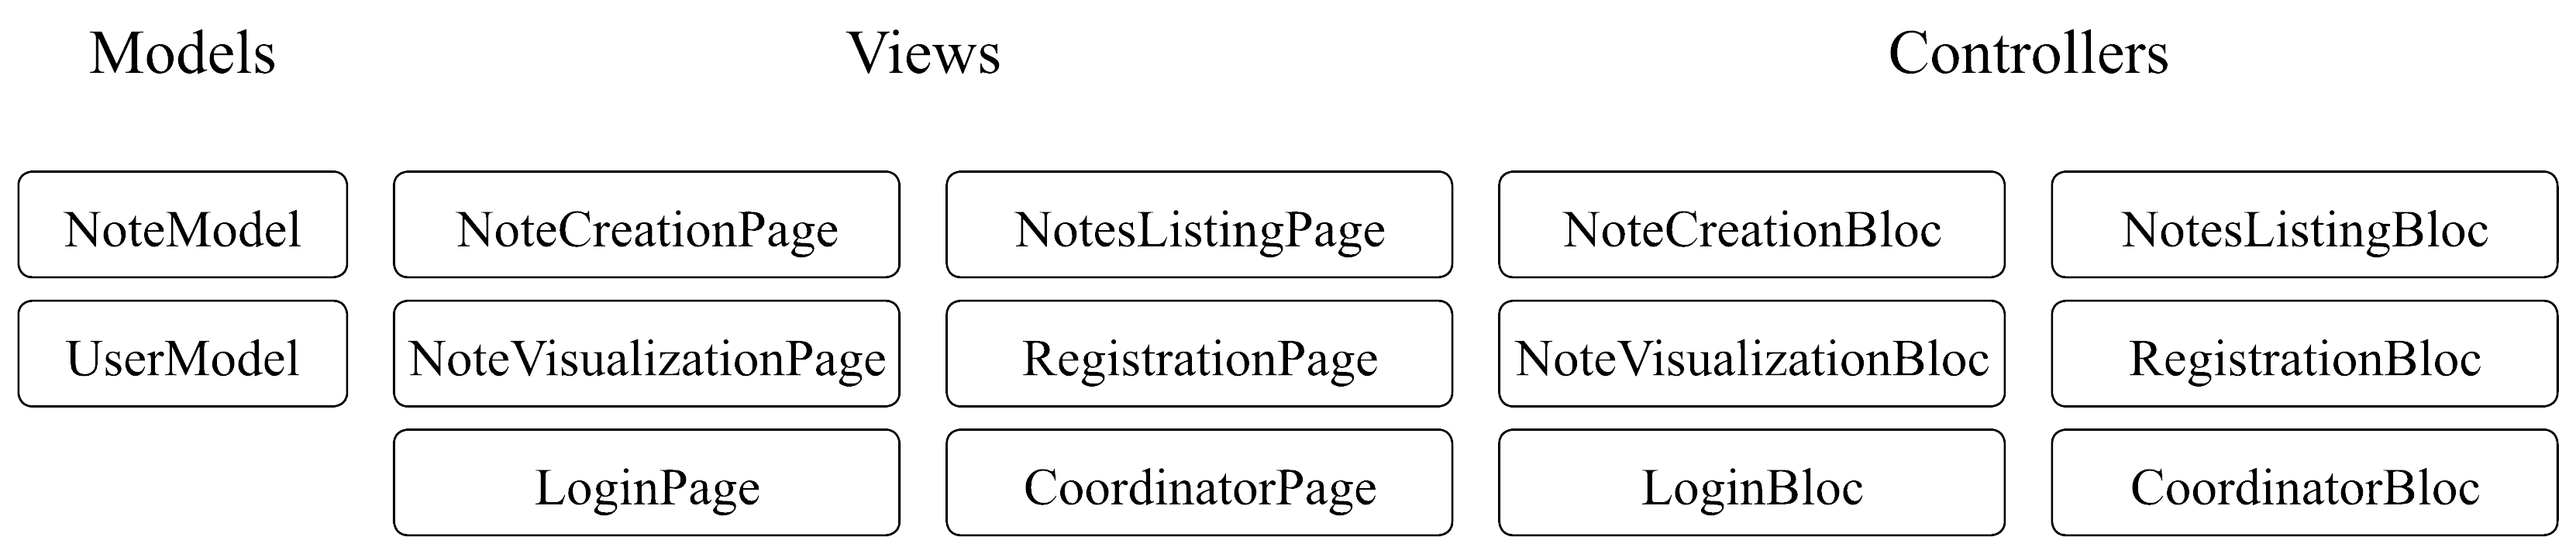
\includegraphics[width=1\textwidth]{images/project_mvc.png}
	\caption{Diagrama do projeto criado com MVC}
	\label{fig:project_mvc}
\end{figure}